\subsection{Vinculación del lector}

Tras conectar el lector a nuestra red WiFi como se explica anteriormente, lo que se muestra en la pantalla de nuestro lector \emph{Arduino} es un mensaje indicando que se necesita vincular el dispositivo.

\begin{figure}[H]
    \centering
    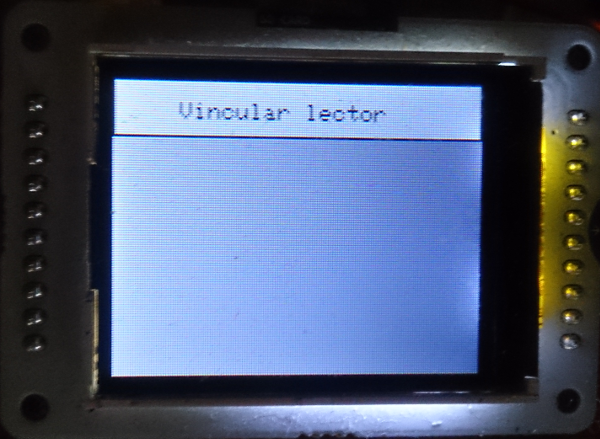
\includegraphics[keepaspectratio,width=0.6\textwidth]{lector_vincular_lector.png}
    \caption{Vincular lector}\label{fig:lector_vincular_lector_1}
\end{figure}


A través de la aplicación web se debe añadir un lector y generar los dos códigos de barras, los cuales se imprimirán para que puedan ser leídos por el lector de código de barras.

Se escanearán con el lector en el orden que se indica en la aplicación web, una vez se han escaneado el lector lanzará una petición para vincularse con nuestra cuenta de usuario. Si el servidor response correctamente, se guarda en la memoria \emph{MicroSD} la clave de acceso pública y se muestra la Home del dispositivo con las opciones disponibles.

En caso de producirse un error se muestra un mensaje para que lo vuelva a intentar.